The capability of searching (querying) on a relational system, was first introduced by Edgar Codd's relational model \cite{codd1970relational} in the 1970s. This model is often referred to when talking about the \ac{sql} model, which appeared shortly after and was loosely based on it. The \ac{sql} model~\cite{Chamberlin:1974:SSE:800296.811515} has almost the same structure of the relational model, with the difference that it added a querying language, \ac{sql}, that has since become a \emph{de facto} standard.

In the late 1990's, relational models went from big, monolithic entities to individual users, this made it necessary for them to be more modular and easier to set up. In this context, \acp{rdbms} where at the basis of every dynamic web page available on the Internet. 

Since then, and for most of the web sites today, this way of storing data is still the best and the one with more development and improvement done through the years. However, a new kind of web sites such as social networks (Facebook\footnote{\url{www.facebook.com}}), that are intended to withstand the visit of thousands of clients simultaneously, making it hard to serve all requests with a relational database without a lot of tuning performed by experts. These social networks give much greater importance to the fact the the service is available at all times than to the clients being able to read the last version of such data, since in this use case most of the data is not sensible and different clients can see different sates of that data without compromising the system. This, alongside with an increase in popularity of a new paradigm called cloud computing which is a way to have easy and on-demand increase in computational power with little management and configurational effort, led to the appearance of the \acp{vlsd} which aim to provide the high scalability and availability storing systems these new paradigms needed. 

\acp{vlsd} usually do not use schemas and do not offer complex queries, as joins. They also attempt to be distributed, horizontal scalable, i.e. as machines are added the performance improves, have easy replication support, which means that data will be stored in more than one machine in order to provide availability and partition tolerance. This comes at the cost of providing weak consistency guarantees, because as Eric Brewer's CAP theorem~\cite{Brewer2000} states, it is impossible for a distributed computer system to simultaneously provide \textbf{consistency}, \textbf{availability} and \textbf{partition tolerance}. For a distributed system to be consistent all clients must see current data regardless of updates or deletes, for it to provide availability, all clients will always be able to read and write data, even with node failures and to be partition tolerant, it must continue to work as expected despite network or message loss.

A typical \ac{rdbms} will focus on availability and consistency, having transactional models that provide what is know as ACID properties, which guarantees that the integrity and consistency of the data is maintained despite concurrent accesses and faults. ACID stands for atomicity, consistency, isolation and durability. 

In this context, \textbf{atomicity} means that a jump from the initial state to the result state will occur without any observable intermediate state, giving all or nothing (commit/abort) semantics that is, when a statement is executed, every update within the transaction must succeed in order to be called successful. To be \textbf{consistent} in a relational model scenario means that the transaction is a correct transformation of the state, i.e only consistent data will be written to the database. \textbf{Isolation} is a property that refers to the fact that no transaction should be able to interfere with another transaction, the outside observer sees the transactions as if they execute in some serial order or in other words, if two different transactions attempt to modify the same data at the same time, then one of them will have to wait for the other to complete. The final property is \textbf{durability} which states that once a transaction commits (completes successfully), it will remain so and that the only way to get rid of what a committed transaction has done is to execute an inverse transaction (which is sometimes impossible) thus, a committed transaction will be preserved through power losses, crashes and errors.  

On the other hand, most \acp{vlsd} focus on availability and partition tolerance (Fig. \ref{fig:cap}), relaxing the consistency guarantee, providing eventual consistency~\cite{Vogels2008}. 

\begin{figure}[htb]
  \begin{center}
    \leavevmode
    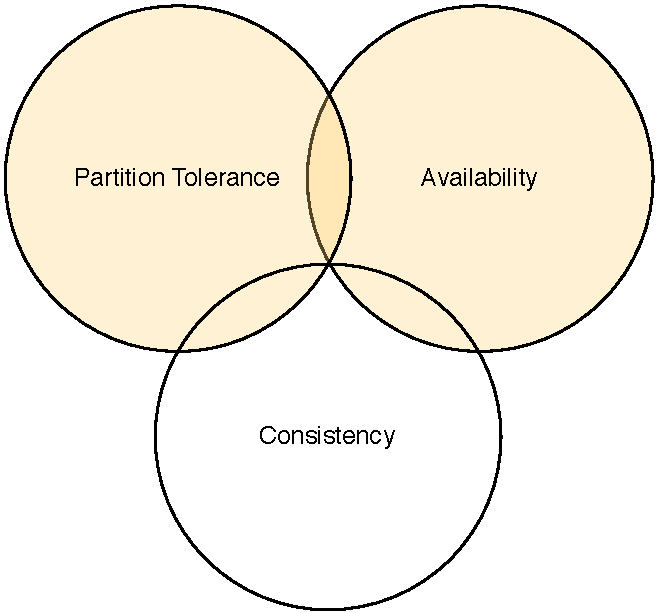
\includegraphics[width=0.5\textwidth]{images/cap}
  \end{center}
  \caption{CAP Theorem}
  \label{fig:cap}
\end{figure}

Eventual consistency means that the storage system guarantees that if no new updates are made to the object, eventually (after the inconsistency window closes) all accesses will return the last updated value. It is seen by many as impracticable for sensitive data, since there is no synchronization that guarantees that updated value will be available at the time of reading. The reality is not so black and white, and the binary opposition between consistent and non consistent is not truly reflected in practice, there are instead degrees of consistency such as strong or causal consistency~\cite{Vogels2008}.

So, on one hand there is the \ac{vlsd} approach, which offers higher scalability, meaning that it can take advantage of having more machines to be able to maintain or even increase its level of performance under bigger loads. On the other hand, a \ac{rdbms} offers more consistency as well as much more powerful query capabilities, leveraging a lot of knowledge and expertise gained over the years \cite{stonebraker2010sql}.  

\section{Problem Statement}

\begin{quote}
If you want to work with a lot of data and be able to run dynamic ad-hoc queries on it, you use a relational database with \ac{sql}. Using a key value store doesn't make any sense for that unless you want to easily be able to distribute your workload on several machines without having to go though the hassle of setting up a relational database cluster. If you want to just keep your objects in a persistent state and have high-performance access to them (e.g. a LOT of web applications), use a key value store.
\end{quote} 
\begin{flushright}in \url{http://buytaert.net/nosql-and-sql}, 25/11/2010\end{flushright}

This separation happens due to the fact that \acp{vlsd} do not provide strong consistency in order to provide partition tolerance and availability, so important in scalable systems. Their reduced \ac{api} makes it simpler and faster to do operations such as a \emph{get} or a \emph{put}. Also, they are prepared from the ground up to replicate data through various machines and even data warehouses.

However, they also have disadvantages as the lack of a standardized query language such as \ac{sql}, making the code vendor specific which in turn makes it less portable. Their simple \ac{api} makes it harder to perform more complex queries and sometimes even impossible since the data is replicated, which makes it hard to maintain an update order and to provide a transactional system with ACID properties. 

These, alongside with the dynamic or non existent schema of these databases, are the main reasons why it is very hard to migrate data and code from a relational database. This kind of migration would save a lot of time and money for companies with huge amounts of code and work done upon relational databases that wish to experience a different type of data storage system.

\section{Objectives}

Migration of data and code is, therefore, something unwanted by developers and managers since it will incur into costs for both, of time and money, respectively. 

According to a blog post by Michael Stonebraker~\cite{stoneEnter}, 61\% of enterprise users are either ignorant about or uninterested in NoSQL\footnote{\acp{vlsd} are subset of NoSQL, since NoSQL does not enforce databases to be distributed}. This happens mainly due to three reasons, because it \textbf{does not provide ACID}, it has a \textbf{low level interface} instead of a high-level language as \ac{sql} and because there is \textbf{no standard} for NoSQL interfaces.

There have been some attempts to make database code the less vendor specific as possible, such as polyglot \acp{orm}\footnote{An orm that outputs different code, according to the database in use, in spite of receiving the same input} as Ruby's DataMapper \cite{DM}, an approach that comes from the fact that even \ac{sql} may differ from \ac{rdbms} to \ac{rdbms} in certain aspects. This portability, however, carries an overhead since it must translate the code to the specific \ac{sql} subset of the required \ac{dbms}.

One problem that \acp{orm} do not solve is migrating legacy \ac{sql} code to a different data model, such as to a \ac{vlsd}. It is exactly this problem that this work aims to tackle, by building a thin layer between the \ac{sql} engine's interpreter and processor, and the actual database underneath it, providing a way to run \ac{sql} queries on top of a \ac{vlsd}.

Alongside with this problem comes another that arise from the limitations of a \ac{vlsd} which is the fact that there is no mechanism to encompass transactions in a \ac{vlsd} and consequently provide the desired ACID properties, which is a problem that this work also addresses and proposes to solve.

To summarize, this work aims:

\begin{itemize}
	\item Allow legacy \ac{sql} code migration to a \ac{vlsd}, taking advantage of a standard language to serve as interface
	\item Provide transactional functionality to the underlying \ac{vlsd}
\end{itemize}

\section{Contributions}

This thesis proposes to provide full \ac{sql} functionality over \ac{vlsd} by altering the \ac{rdbms} underlying storage system.
The major factor in this implementation is that it takes advantage of the scalability and replication features from the \ac{vlsd}, and allies them with the \ac{rdbms} \ac{sql} engine. Also, it provides a completely separate library for transactions in a \ac{vlsd}. 

In detail, we make the following contributions:

\begin{itemize}
	\item \textbf{Prototype database system providing full \ac{sql} functionality over \ac{vlsd}}\\
	   We developed a prototype that allows for \ac{sql} queries to be run over a \ac{vlsd}. In detail, we ported the Apache Derby's query engine to use the Cassandra \ac{vlsd} as its storage layer.
		
	\item \textbf{Distributed transactions library for a \ac{vlsd}}\\
		We developed a library that allows to create and manage transactional contexts enabling to ensure ACID guarantees. 
		
	\item \textbf{Evaluation of the proposed solution}\\
		We evaluate the developed solution using the TPC-W benchmark~\cite{tpcw}, analyzing its behavior under different conditions and configurations comparing its performance to that of a standard \ac{rdbms}. We also evaluated it using the \ac{ycsb} in order to measure the performance of the transactions library without Derby's query engine.
\end{itemize}


\section{Dissertation Outline}

This thesis is organized as follows: Chapter 2 describes the main features of most \acp{vlsd} and some of the implementations; Chapter 3 introduces \ac{sql} and its main functionalities; Chapter 4 describes the modifications made to both Derby and Cassandra in our implementation; Chapter 5 introduces the proposed solution for distributed transactions for \acp{vlsd}; Chapter 6 evaluates the solution implemented using realistic workloads; Chapter 7 describes the related work; and finally Chapter 8 concludes the thesis, summarizing its contributions and describing possible future work. 
